\chapter{Possible Fertilisation of Mbona Trout Eggs}
 
 Currently, Mbona purchases pre-fertilised eyed eggs for their hatching trays. However it may be possible to
 strip and fertilise our own fish if we have a reasonable collection of mature female and male trout.
 These brood fish should ideally be about 3 years old. In this chapter we outline what would be required in order to accomplish this operation. These recommendations come from Gavin Chin.
 
 \section{Infrastructure}
 
 \subsection{Housing}
 Fertilised Eggs must be incubated in a "tower" that remains undisturbed in the dark for at least
 25 days. To accommodate this tower the Mbona hatcheries must purchase another shed to house the
 incubation tower. This shed can be small as only one tower is envisaged. Probably a "guard hut" residing
 on a concrete base will do.
 
\subsection{Egg towers}

The newly fertilised eggs must reside undisturbed in a {\bf tower} for about 25 days. This tower has the
following properties, see diagram in figure \ref{fig:FertilisationTower}.

\begin{figure}[H]
  \centering
   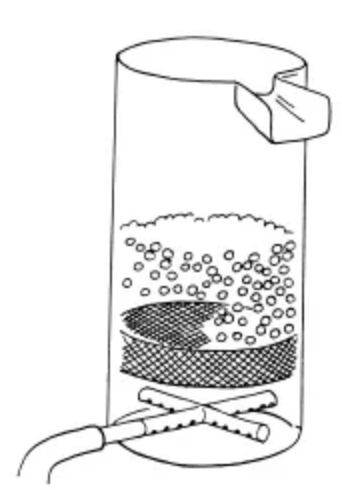
\includegraphics[scale = 0.5]{images/FertilisationTower.png}
  \caption{Fertilisation Tower.}
   \label{fig:FertilisationTower}
\end{figure}



                  \begin{itemize}
                  \item  Egg towers to stand on concrete base set through cabin floor. 
                  \item 75mm PVC tube, castellated top with light-proof lid set in 35mm thick concrete base
                  \item gravel chip diffuser, stainless steel mesh above, 
                  \item 1/2inch inlet with tee for vertical anti bubble pipe.  
                  \item Hypodermic needle set into clear plastic inlet pipe for Malachite infusion.
                  \end{itemize}
                  
 
\section{Stripping Equipment}

\begin{itemize}
\item table  
\item towel  
\item paper towel 
\item 2  large bowls  
\item 2 jars 
\item wet cloth  
\item smooth anorak 
\item one teaspoon 
\item one long feather
\item 2  large nets  
\item recovery tank with good oxygenated water
\item 2l malachite solution
\item egg tower with constant supply of oxygenated water.
\end{itemize}

\subsubsection{Malachite solution: }

                  \begin{itemize}
                  \item 2l water (preferably preboiled)
                  \item 1 x heaped teaspoon Zink free Malachite powder (Supplier details from Gavin)
                  \item Keep solution in sealed bottle.
                  \end{itemize}


\section{Workers}
\begin{itemize}
\item fish catcher 
\item runner 
\item fish stripper  
\item an assistant 
\item fish recoverer
\end{itemize}

                                       

\section{Method}

\subsection{Stripping the Hens}   

\begin{itemize}
\item Make sure both stripping bowls are completely dried using paper towel. 
Any water mixed into the eggs at this stage would result in the eggs not being fertilised.
\item Presuming the stripper is right handed, use the wet cloth to hold fish by the tail in left hand. 
\item Tuck the fish's head under your left arm hiding its eyes, (vent away from yourself).
\item Using the towel,  ask the assistant is to dry the nipple area of the fish in the direction of the tail. 
\item Strip each hen into the smaller dried bowl so that ova can be assessed.
\item Only when seen to be NOT haloed add ova to larger bowl.
\item Using the right hand the stripper milks the fish on the underbelly to expel the eggs. 
\item It may take a few strokes before the eggs appear.
\item If the belly is hard and no eggs appear, then the fish is not ready and goes in the recovery tank. 
\item If the eggs are haloed (ie translucent with an orange dot), then the eggs are too old and must not be mixed in with the other eggs. If even one egg in a batch is haloed, throw the entire batch away, but continue to strip the fish or she may become egg-bound and die. 
\item If last years eggs are expelled with good eggs, they must be removed with the teaspoon. They appear as a whitish shell.The eggs should be uniform orange in colour. 
\item Strip the fish until all eggs are out.  If the fish defecates during stripping (black  in colour), remove the faeces using the teaspoon. 
\item If the fish tenses, allow her to relax before continuing stripping. 
\item If she struggles, allow her to drop gently to the table then continue with the process.  
\end{itemize}
 
\subsection{Recovery}

\begin{itemize}
\item Take fish to recovery tank as soon as possible
\item Hold her upright under the water and closest to oxygenated water while cleaning off her body the slime
that has built up during stripping.
\item Only the slime that occured during stripping to be removed to prevent her getting a fungus.
\item Keep holding her upright until she swims away out of your hands. 
\item Do not pull her backwards through the water. 
\item The person aiding fish to recover must stand at the tank and check for fish turning on their side. 
\item The fish must be helped to remain upright to make a full recovery. 
\item Return recovered fish to their own tank within a couple of hours. 
\end{itemize}

\subsection{Stripping the Cocks}

\begin{itemize}
\item Once the females have been stripped, the catcher sends a male to be held in the same way. 
\item The milt from the male is to be stripped into one of the jars. 
\item Remove faeces if necessary. 
\item One or two males may be enough for fertilisation. 
\end{itemize}

\subsection{Fertilisation}

\begin{itemize}
\item Pour the milt into the eggs. 
\item Stir very gently with a feather until eggs are coated with milt.
\item Leave for about 10 minutes
\item Add water to the bowl until the bowl is a third to a half full. 
\item Leave for half an hour.
\item Cover to prevent light entering.
\item Flush eggs with clean water and remove dead (white) eggs.
\item Add to the tower, through which a constant supply of oxygenated water is flowing. 
\item Leave in tower overnight.
\item Next morning, pour ova into bowl with water and remove all dead eggs and replace in tower.
\item Leave for 4 days undisturbed. 
\item After 4 days treat eggs by injecting 10ml of malachite solution daily to prevent fungal infection.  
\item When eyed after about 25 days transfer to egg trays.
\end{itemize}

    

